%!TEX root = ../thesis.tex

% *****************************************************************************
% ********************************** CHAPTER 3 ********************************
% *****************************************************************************

\chapter{Publish/Subscribe communication}

Publish/subscribe (pub/sub) technology encompasses a wide number of solutions
that aim at solving a vital problem pertaining to timely information
dissemination and event delivery from publishers to subscribers.
\cite{Pub/Sub_pattern}

In a pub/sub system there are two entities which can participate to the
communication: the publishers and the subscribers.
Subscribers have the possibility to express their interest in a type of event
or a pattern of event, and they are notified when a publisher generate an event
which they are interested in.

The biggest advantage in using pub/sub communication is the decoupling of
in space, time and synchronization between publishers and subscribers.
\cite{Many_faces_of_pub/sub}

The pub/sub paradigm is very useful in describing and monitoring the world
around us. Any person meets a constant barrage of events in his 


\section{Apache Kafka}

Apache Kafka is an open-source distributed even streaming platform that can
publish, subscribe to, store, and process streams of records in real time.
It is designed to handle data streams from multiple sources and deliver them to
multiple consumers. \cite{garg2013apache}

\begin{figure}[ht]
    \centering
    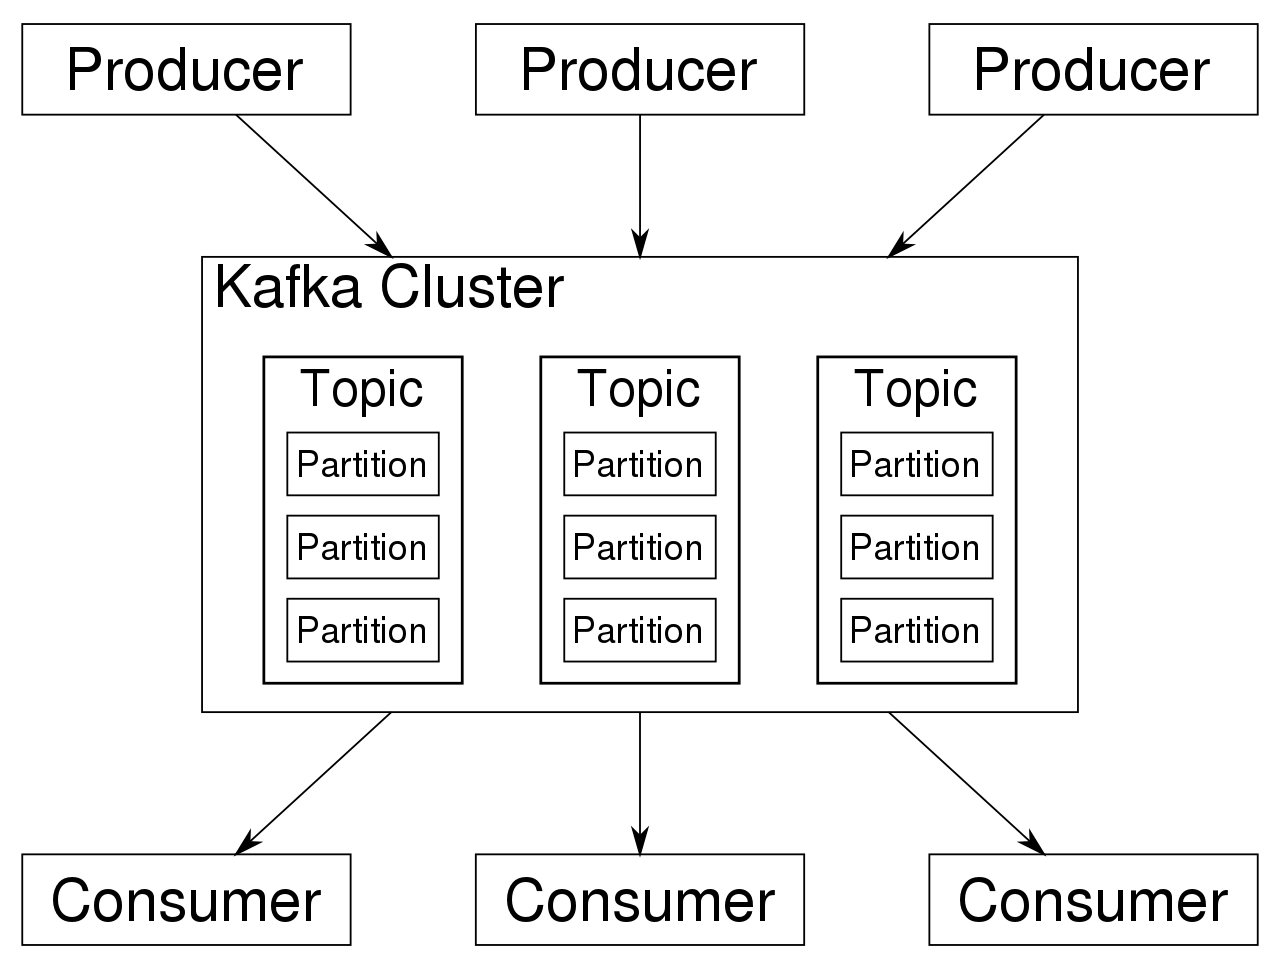
\includegraphics[width=1.0\textwidth]{kafka_architecture.png}
    \caption{Apache Kafka Architecture}
\end{figure}

The main characteristics of Kafka are:

\begin{enumerate}
    \item   Persistent messaging: the messages are not lost, at least until
            they are read.
    \item   High throughput: Kafka support millions of messages per second.
    \item   Distributed: Kafka support distributing consumption over a cluster
            of consumer machines while maintaining ordering semantics.
    \item   Multiple client support: Kafka supports the integration of clients
            from different platforms.
    \item   Real Time: Messages produced by the threads should be immediately
            visible to consumers.
\end{enumerate}

Kafka is a distributed system consisting of servers and clients that
communicate via a high performance TCP network protocol.  It can be deployed
on bare-metal hardware, virtual machines, and containers in on-premise as well
as cloud environments.

Kafka is run as a cluster of one or more servers that can span multiple
datacenters or cloud regions. Some of these servers form the storage layer,
called brokers. For mission critical use cases, a Kafka cluster is highly
scalable and fault-tolerant: if any of its servers fails, the other servers
will take over their work to ensure continuous operations without any data
loss.

Kafka clients allow to write distributed applications and microservices that
read, write and process streams of events in parallel, at scale, and in a fault
tolerant manner even in the case of network problems or machine failures.

\subsection{Events}

Events are one of the most important elements in Kafka.
An event records the fact that "something happened". When data is written or
read, this is done in form of events in Kafka. \cite{kafka_documentation}

Event streaming is the practice of capturing data in real-time from event
sources like databases, sensors, mobile devices, cloud services, and software
applications in the form of of streams of events; storing 

An evet has a key, value, timestamp and optional metadata headers. An example
of event could be:

\begin{itemize}
    \item   Event key: "Alice"
    \item   Event value: "Made a payment of \$200 to Bob"
    \item   Event timestamp "Jun. 25, 2020 at 2:06 p.m."
\end{itemize}

\subsection{Topics}

In every messaging system based on pub/sub communication, the topic plays one
of the most important role, providing the possibility to decouple consumers
and producers.

Events, or messages, are organized and durably stored in topics.
Topics in Kafka are always multi-producer and multi-subscriber.
Events in a topic can be read as often as needed, unlike traditional messaging
systems, events are not deleted after consumption. Instead, you define for how
long Kafka should retain your events through a pre-topic configuration setting,
after which old events will be discarded. Kafka's performance is effectively
constant with respect to data size, so storing data for a long is perfectly

\subsection{Partitions}

Topics are partitioned, meaning a topic is spread over a number of "buckets"
located on different Kafka brokers.
This distributed placement of your data is very important for scalability
because it allows client appliations to both read and write the data from/to
many brokers at the same time. When a new event is published to a topic, it is
actually appended to one of the topic's partitions.

\begin{figure}[ht]
    \centering
    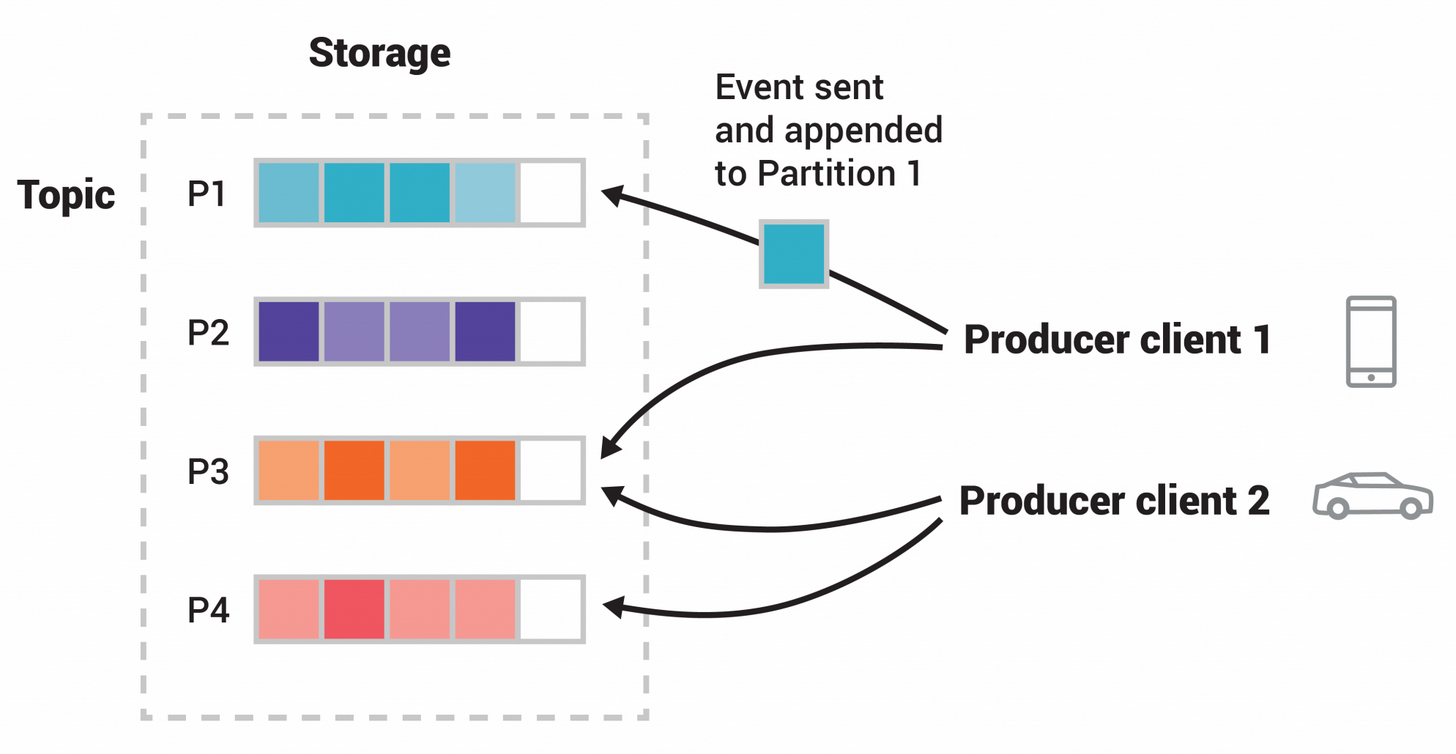
\includegraphics[width=1.0\textwidth]{kafka_partitions.png}
    \caption{Kafka Partitions}
\end{figure}

Everything in Kafka is modeled around partitions. They rule Kafka's storage,
scalability, replication and message movement.

Kafka's topics are divided into several partitions. While the topic is a
logical concept in Kafka, a partition is the smallest storage unit that holds
a subset of records owned by a topic. Each partition is a single log file
where records are written to it in an append-only fashion.

\begin{figure}[ht]
    \centering
    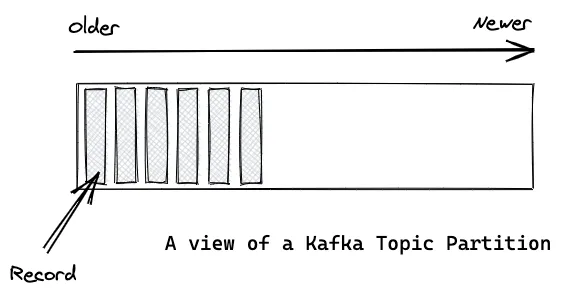
\includegraphics[width=1.0\textwidth]{kafka_partition2.png}
    \caption{Structure of a partition}
\end{figure}

\subsubsection{Offsets}

The records in the partitions are each assigned a sequential identifier
called the offset, which is unique for each record within the partition.
The offset is an incremental and immutable number, maintained by Kafka.
When a record is written to a partition, it is appended to the end of the log,
assigning the next sequential offset.

Offsets are used by consumers when reading records from a partition.

\begin{figure}[ht]
    \centering
    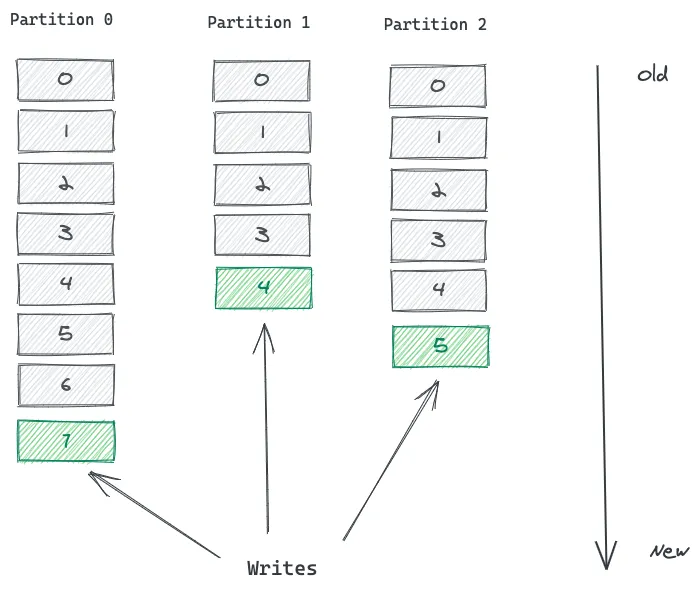
\includegraphics[width=1.0\textwidth]{kafka_partition3.png}
    \caption{Partitions with the offset for every record}
\end{figure}

Although messages within a partition are ordered, messages across a topic are
not guaranteed to be ordered.

For every consumer, Kafka only needs to maintain the information about the
latest offset.

\subsubsection{Distribution of Partitions}

A Kafka cluster is made of one or more servers. In the Kafka universe, they are
called brokers.
Each broker holds a subset of records that belongs to the entire cluster.
Kafka distributes the partitions of a particular topic across multiple brokers.

To make your data fault-tolerant and highly available, every topic can be
replicated, even across geo-regions or datacenters, so that there are always
multiple brokers that have a copy of the data just in case things go wrong, you
want to do maintenance on the brokers, and so on.
Replication is done at the partition level.

Advantages:

\begin{itemize}
    \item   By spreading partitions across multiple brokers, a single topic can
            be scaled horizontally to provide performance far beyond a single
            broker's ability.
    \item   A single topic can be consumed by multiple consumers in parallel.
    \item   Serving all partitions from a single broker limits the number of
            consumers it can support. Partitions on multiple brokers enable
            more consumers.
    \item   Mutliple instances of the same consumer can connect to partitions
            on different brokers, allowing very high message processing
            throuhgput.
\end{itemize}

The copies of the partitions are called replicas. If a broker fails, Kafka
can still serve consumers with the replicas of partitions that failed broker
owned.

Kafka replicate partitions so if a broker goes down, a backup partition takes
over and processing can resume. The replication factor is configurable
(e.g., configurable factor of three creates three copies of a partition, one
leader and two followers).

All reads and writes go to the leader of the partition. Typically, there are
many more partitions than brokers and the leaders are evenly distributed among
brokers. The logs on the followers are identical to the leader's log; all have
the same offsets and messages in the same order. Although at any given time,
the leader may have a few unreplciated messages at the end of its log.

Followers consume messages from the leader like a Kafka consumer would and
apply them to their own log. Followers pulling from the leader enables the
follower to batch log entries applied to their log.

\subsection{Producers}

Producers in Apache Kafka serve as data publishers, sending messages or events
to topics within the Kafka cluster.
The producer is \textit{thread safe} and sharing a single producer instance
across threads will generally achieve better performance than having multiple
instances.

\begin{figure}[ht]
    \centering
    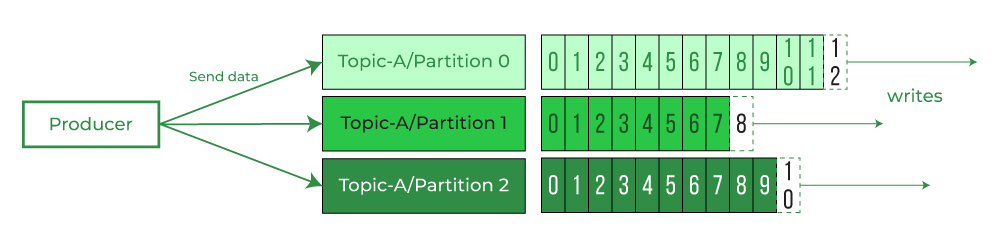
\includegraphics[width=1.0\textwidth]{kafka_producer.png}
    \caption{Example of Producer publishing data}
\end{figure}

The producer consists of a pool of buffer space taht holds records that haven't
yet been transmitted to the server as well as a background I/O thread that is
responsible for turning these records into requests and transmitting them to
the cluster.

The \textbf{send()} method is asynchronous. When called it adds the record to a
buffer of pending record and returns immediately. This allows the producer to
batch together individual records for efficiency.

The producer maintains buffers of unsent records for each partition. The batch
size is configurable, to satisfy the need of every application. Making the
batch size larger can result in an improvement in efficiency, but it requires
more memory.

\subsubsection{Fault Tolerance}

The producers in Kafka will automatically know to which broker and partition to
write based on the message and in case there is a Kafka broker failure in the
Kafka cluster, the producers will automatically recover from it, which makes
Kafka resilient and highly adaptable.

\subsubsection{Load Balancing}

The producer sends data directly to the broker that is the leader for the
partition without any intervening routing tier. To help the producer do this,
all Kafka nodes can answer a request for metadata about which servers are alive
and where the leaders for the partitions of a topic are at any given time to
allow the producer to appropriately direct its requests.

The producer controls which partition it publishes messages to. This can be
done at random, implementing a random load balancing, or it can be done by a
semantic partitioning function.
This second approach allows the developer to define a partition key and use it
together with an hashing function to decide to which partition publish the
message (e.g., if the key chosen was a user id, then all data for a given user
would be send to the same partition).

Messages written to the partition leader are not immediately readable by
consumers regardless of the producer's acknowledgement settings.
When all in-sync replicas have acknowledged the write, then the message is
considered committed, which makes it available for reading.
This ensure taht messages cannot be lost by a broker failure after they have
already been read. This implies that messages which were acknowledged by the
leader only can be lost if the partition leader fails before the replicas have
copied the message. Nevertheless, this is often a reasonable compromise in
practice to ensure durability in most cases while not impacting throughput too
significantly.

\subsubsection{Asynchronous Send}

Batching is one of the big drivers of efficiency, and to enable batching the
Kafka producer will attempt to accumulate data in memory and to send out
larger batches in a single request. The batching can be configured to
accumulate no more than a fixed number of messages and to wait no longer than
some fixed latency bound. This allows the accumulation of more bytes to send,
and few larger I/O opeartions on the servers. This buffering is configurable
and gives a mechanism to trade off a small amount of additional latency for
better throughput.

\subsection{Consumers}

Consumers are vital components that subscribe to specific topics within Kafka
cluster to retrieve and process messages or events. They play a key role in
data consumption, allowing applications to access and utilize the information
published by producers, facilitating real-time data processing and analysis.
They work by issuing "fetch" requests to the brokers leading the partitions it
wants to consume.
The consumer specifies its offset in the log with each request and receives
back a chunk of log beginning from that position.
The consumer has significant control over this position and can rewind it to
re-consume data if needed.

\subsubsection{Push vs Pull}

In this respect, Kafka follows a more traditional design, shared by most
messaging systems, where data is pushed to the broker from the producer and
pulled from the broker by the consumer.
A push based system has difficulties dealing with different consumers as the
broker controls the rate at which data is transferred.

A pull based system has the nicer property that if the consumer falls behind 
in processing messages, it can catch up at any time.
Another advantage of a pull-based system s that it lends itself to aggressive
batching of data sent to the consumer. A push-based system must choose to
either send a request immediately or accumulate more data and then send it
later without knowledge of whether the downstream consumer will be able to
immediately process it. If tuned for low latency, this will result in sending
a single message at a time only for the transfer to end up being buffered
anyway, which is wasteful.
A pull-based design fixes this as the consumer always pulls all available
messages after its current position in the log. Optimal batching is achieved
without introducing unnecessary latency.

\subsubsection{Consumer Position (Offset)}

Keeping track of \textit{what} has been consumed is one of the key performance
points of a messaging system.

A topic is divided into a set of totally ordered partitions, each of which is
consumed by exactly one consumer within each subcribing consumer group at any
given time.
This means that the position of a consumer in each partition is just a signle
integer: the offset of the next message to consume.
This makes the state about what has been consumed very samll, just one number
for each partition. This state can be periodically checkpointed. This makes the
equivalent of message acknowledgments very cheap.

There is a side benefit of this decision. A consumer can deliberately rewind
back to an old offset and re-consume data. This violates the common contract of
a queue, but turns out to be an essential feature for many consumers.

\subsubsection{Detecting Consumer Failure}

After subscribing to a set of topics, the consumer will automatically join the
group when \textit{poll(Duration)} is invoked.
The poll API is designed to ensure consumer liveness. As long as you continue
to call poll, the consumer will stay in the group and continue to receive
messages from the partitions it was assigned. Underneat the surface, the
consumer sends periodic hearbeats to the server. If the consumer creashes or is
unable to send heartbeats for a configured duration, then the consumer will be
considered dead and its partitions will be reassigned.

\subsection{Brokers}

Kafka cluster consists of one or more servers, called brokers, which execute
Kafka. Using a single broker for an application is possible, but it doesn't
allow to exploit all the services that Kafka offers, like data replication.

\subsection{Writing Records to partitions}

There are three different ways that a producer can write a record to a
partition:

\begin{itemize}
    \item   Partition key
    \item   Kafka decides the partition
    \item   Writing to a customer partition
\end{itemize}

\subsubsection{Partition key}

A producer can use a partition key to direct messages to a specific partition.
A partition key can be any value that can be derived from the application
context (e.g., device ID, user ID).

By default, the partition key is passed through a hashing function, which
creates the partition assignment. That assures that all records produced with
the same key will be located in the same partition. Specifying a partition key
enables keeping related events together in the same partition and in the exact
order in which they were sent.

\begin{figure}[ht]
    \centering
    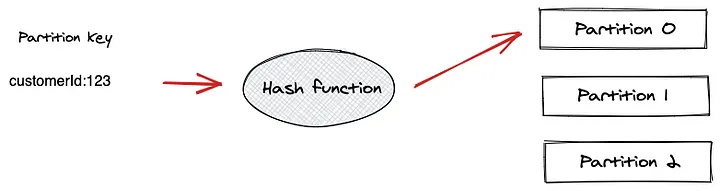
\includegraphics[width=1.0\textwidth]{kafka_partition_key.png}
    \caption{Distribution of messages based on partition key}
\end{figure}

The data distribution of the partition key can lead to broker skew if keys are
not well distributed. It's important to use a partition key to put related
events together in the same partition in the exact order in which they were
sent.

\subsubsection{Kafka decide the partition}

If a producer doesn't specify a partition key when producing a record, Kafka
will use a round-robin partition assignment. Those records will be written
evenly across all partitions of a particular topic.
However, if no partition key is used, the ordering of records can not be
guaranteed within a given partition.

\subsubsection{Writing a customer partition}

In some situations, a producer can use its own partitioner implementation that
uses othre business rules to do the partition assignment.
This guarantees the maximum customization, satisfying all the needs an
application can have.

\subsection{Reading records from a partition}

Unlike the other pub/sub implementations, Kafka does not push messages to
consumers.
Instead, consumers have to pull messages off Kafka topic partitions. A consumer
connects to a partition in a broker, reads the messages in the order they were
written.

The offset of a message works as a consumer side cursor at this point.
The consumer keeps track of which messages it has already consumed by keeping
track of the offset of messages. After reading a message, the consumer advances
its cursor to the next offset in the partition and continues.
Advancing and remembering the last rewad offset within a partition is the
responsability of the consumer.

By remembering the offset of the last consumed message for each parititon, a
consumer cna join a partition at the point in time they choose and resume from
there. That is particularly useful for a consumer to resume reading after
recoverting from a crash.

\begin{figure}[ht]
    \centering
    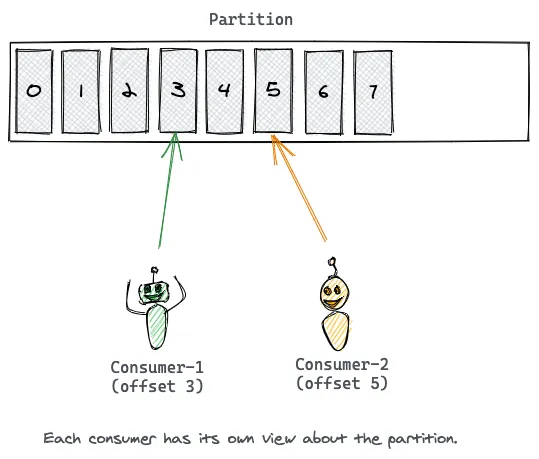
\includegraphics[width=1.0\textwidth]{kafka_reading_partitions.png}
    \caption{Example of reading a partition from two consumers}
\end{figure}

\subsection{Consumer Groups}

Kafka has the concept of consumer groups where several consumers are grouped
to consume a given topic. Consumers in the same consumer group are assigned the
same group-ID value.

The consumer group concept ensures that a message is only ever read by a single
consumer in the group.

Multiple consumer groups are useful when different applications need to read
the same content. Each consumer would have different offset pointer to keep
information about the latest read record.

When a consumer group consumes the partition of a topic, Kafka makes sure that
each partition is consumed by exactly one consumer in the group.

\begin{figure}[ht]
    \centering
    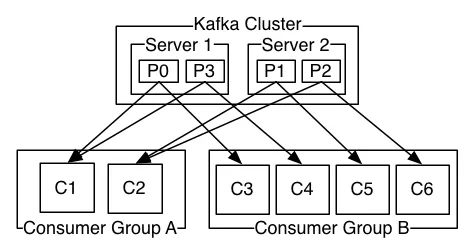
\includegraphics[width=1.0\textwidth]{kafka_consumer_group.png}
    \caption{Consumer groups reading from the Kafka cluster}
\end{figure}

Consumer groups enalb econsumer to parallelize and process messages at very
high throughputs. However, the maximum parallelism of a group will be equal to
the number of partitions of that topic.

\begin{figure}[ht]
    \centering
    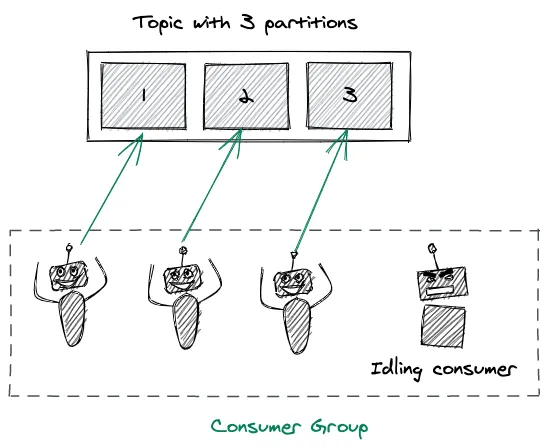
\includegraphics[width=1.0\textwidth]{kafka_parallelism.png}
    \caption{Kafka degree of parallelism}
\end{figure}

The number of consumers don't govern the degree of parallelism of a topic.
It's the number of partitions that governs the degree of parallelism.

\subsection{Acks}
